\section{Konzept 3}
F\"{u}r dieses Konzept wird ein industrieller Aerosolgenerator verwendet, dessen Partikelstrom in einem Container konzentriert wird, um von dort aus einen Partikelsprung zu generieren.
\subsection{Aufbau}
Die Versuchseinrichtung besteht aus einem Aerosolgenerator, einem gro{\ss}en Container, dem ausgew\"{a}hlten Schiebersystem und dem Messger\"{a}t. F\"{u}r die Verbindung zwischen Generator und Container wird ein Schlauch verwendet. Ein Rohr bildet die Schnittstelle zwischen dem Aerosolauslass des Containers und des Schiebersystems und ein weiteres Rohr dient zur Aufnahme der Umgebungsluft, welches auch zum Schiebersystem f\"{u}hrt. Die Verbindung zum Messger\"{a}t ist anschlie{\ss}end mit einem kurzen Rohr gel\"{o}st.
\begin{figure}[H]
        \myfloatalign
        {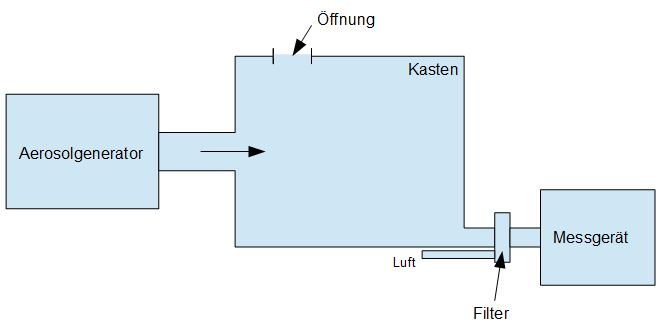
\includegraphics[width=.9\linewidth]{gfx/concepts/Konzept_3.jpg}} \quad
        \caption[Skizze Konzept 3]
        {Skizze Konzept 3}
        \label{fig:concept_3}
\end{figure}

\subsection{Funktionsweise}
Das Messger\"{a}t saugt w\"{a}hrend der Aerosolherstellung Umgebungsluft, welche \"{u}ber einen Filter gereinigt wird. Das Schiebersystem befindet sich hierbei in der \textit{Stellung 0}. W\"{a}hrend der Aerosolherstellung flie{\ss}t das bereits fertiggestellte Aerosol \"{u}ber einen Schlauch in den gro{\ss}en Container bis dieser gef\"{u}llt ist. Der Aerosolauslass zum Messger\"{a}t ist zu dieser Zeit durch den elektrisch betriebenen Schieber geschlossen (\textit{Stellung 0}). Nach der Fertigstellung schaltet der Schieber den Auslass frei und der Sprung wird mittels Aerosolstrom erzeugt. Die Luftzufuhr ist gestoppt und somit befindet sich das Schiebersystem in \textit{Stellung 1}. Der Schaltvorgang zwischen Luft und Aerosol findet in festen zeitlichen Abst\"{a}nden statt. Das abwechselnde Beaufschlagen von gefilterter Umgebungsluft und Aerosol gew\"{a}hrleistet einen ausreichenden Konzentrationsunterschied, um das generierte Sprungsignal zu verst\"{a}rken.
\\\\
Die Messung startet bereits w\"{a}hrend der Aerosolgenerierung. Um die Verz\"{o}gerungszeit der Schnittstelle, folglich auch die Totzeit des gesamten Systems, so gering wir m\"{o}glich zu halten, wird das Aerosolrohr im Schiebersystem und das Rohr zum Messger\"{a}t sehr kurz gew\"{a}hlt. Die Verz\"{o}gerungszeit ist die Zeit, die das Eingangssignal braucht, um den Weg zum Messger\"{a}t zu \"{u}berbr\"{u}cken inklusive der Schaltzeit des Schiebers. Diese ergibt mit der Totzeit des Messger\"{a}tes die Totzeit des gesamten Systems.
